%# -*- coding: utf-8-unix -*-
% !TEX program = xelatex
% !TEX root = ../thesis.tex

\chapter{Background}

\section{Online Judge}
    
    \subsection{Programming Education}

        As we walk into a century surrounded by all kinds of computing devices,
        programming skill gains more and more attention.
        Universities used to teach programming to merely computer science major students,
        but more and more of them are opening the course to all.

        One part of programming education is mastering one programming language.
        Mechanisms of modern computers may be too complicated for non-computer science majored students to learn,
        but thanks to the abstractions of processors, operating systems, and high-level programming languages,
        it becomes easier and easier to program computers to do what users want.
        The most popular high-level programming languages include C++, Python, Java, and so on.
        Instead of dealing with registers and memory addresses using processors' instruction set,
        high-level programming languages bring up concepts like variables, arrays, expressions, loops, functions,
        threads, processes, and other computer science abstractions.

        The other part of programming education is learning programmatic thinking, in other words,
        algorithms and data structures, especially for computer science majored students.
        There may be several solutions to the same problem, but taking different approaches costs differently.
        An $O(n\log n)$ algorithm better scales to a larger input compared to an $O(n^2)$ algorithm.
        Programming also helps students cultivate thinking skills.
        There are mind sports especially focus on algorithms.
        For instance, ACM International Collegiate Programming Contest (\emph{ACM-ICPC}) is an annual
        competitive programming competition among the universities of the world.
        In 2017, 49,935 students from 3,098 universities in 111 countries participated. \cite{acmicpc_fact_sheet}
        Companies value this kind of thinking skills, as well.
        It is a common practice for companies to ask algorithm puzzles when interviewing candidate programmers.

        Higher level courses in computer science, like Networking, Machine Learning, and so on,
        need students to be able to express their mind in code.
        Therefore, It is crucial for students to master programming at the very beginning of the study,
        which puts challenges to entry-level courses, such as Programming Language, Data Structures, and so on.

        Like any other skills, both mastering one programming language and learning programmatic thinking
        require students to practice repeatedly.
        Essential ways of these entry-level courses to help students master programming are assignments and exams.
        Problems in the assignments and exams are likely tasks asking students to write code.
        Graphics interfaces, keyboard and mouse inputs, video and audio outputs, networking connections,
        reading from and writing to disks, and so on, are common operations what programs in end-users' computers would have,
        but it would be too much burden for starters.
        Because these problems are for educational purpose only, the tasks are simplified from the real world ones.

        Descriptions of these problems are simple and neat. The tasks are idealized.
        Students need to deal with neither incorrect inputs nor malicious data.
        Problems are algorithmic in nature, thus there is no need to consider human-computer interaction.
        Memory is assumed to be large enough for the problems, therefore students can avoid disk operations
        and keep everything in memory.
        In a word, these assignments and exams ask students to write code that focuses on the ``computing'' part of programming.

        After students finish the tasks, there need to be some ways to give them feedback, at least,
        tell students whether their solution is correct or not.
        Traditionally, grading programming solutions had no difference from grading calculus homework.
        And the emerge of online judges two decades ago enabled more efficient grading.
        
    \subsection{Manual Grading}

        Before the appearance of online judges, teachers needed to grade programming solutions manually.
        First, students handed in their solutions.
        Then, graders (either the professor himself/herself or the teaching assistants)
        would read the code and give marks based on their professional judgment.
        Manual grading is still a common practice nowadays in other subjects, such as mathematics and physics.
        Though widely used, its effectiveness is still affected by several non-controllable factors
        and has significant drawbacks. \cite{Kurnia2001}

        \subsubsection{Discouragement of Alternative Solutions}

            When the teachers are sketching a problem, they have a standard solution in mind.
            So when graders are grading students' solutions, they expect the code to be similar to
            the standard solution that they were told.
            However, it is likely that there are several alternative solutions to the same problem
            with the same complexity if not better.
            For instance, suppose an assignment can reduce to a minimum spanning tree problem
            and the author expects the Prim algorithm. \cite{cheriton1976finding}
            A student might turn in a solution with Kruskal algorithm which is also an algorithm that
            solves the minimum spanning tree problem. \cite{kruskal1956shortest}
            In this case, if the grader is not aware of Kruskal algorithm, the grader might give a wrong verdict
            because Kruskal algorithm looks utterly different from Prim algorithm, i.e., the standard solution.
            Notice that this is not the fault of the grader, because the grader might be a teaching assistant
            who is only expected to be familiar with the standard solution.
            Neither is this the fault of the problem author because there can be any number of alternative solutions
            and the author cannot enumerate them all.
            Nor should we blame the student.
            On the contrary, students with alternative solutions should be encouraged.

        \subsubsection{Slow Grading}

            Grading a programming solution can take a long time.
            Unlike a solution to mathematics homework in which students will explain their thinking process
            step by step in natural language,
            a solution to a programming problem is code in some programming language which is designed
            for machines to compile, instead of letting humans read.
            The grader has to read the code carefully in order to understand the solution.
            Then they need to look into details trying to find potential mistakes.
            Consequently, the grading process can be prolonged.

        \subsubsection{Inconsistency}

            The same solution might have different scores if a different grader grade it.
            For example, some graders know more than the standard solutions
            and thus justify the alternative solutions.

            Even for the same grader to check the same solution at different times might lead to different results.
            For instance, at the beginning of grading, the grader might be very patient
            and carefully reason about each line of code.
            However, after hours of grading, the grader could feel tired and distracted
            and might want to finish grading as soon as possible.
            In this case, the grader might only check if the solution matches some patterns of the standard solution.

            Needless to say, the same solution is likely to have completely different verdicts
            depending on who the grader is and what status he or she is in.

        \subsubsection{Ignorance of Details Mistakes}

            Because of understanding students' solution costs graders lots of energy,
            subtle mistakes hidden in details often escape from being found.
            For example, supposing the standard solution is Floyd algorithm, \cite{ingerman1962algorithm}
            the grader might expect students' solutions to have two kinds of patterns:
            three nested loops and a dynamic programming equation.
            However, the solution might mix up the permutation of the three loop variables,
            which makes the algorithm no longer correct.
            The grader might not be able to find such subtle an error.

            \begin{lstlisting}[language=Python]
# Correct Algorithm Fragments:
for k in range(len(V)):
    for i in range(len(V)):
        for j in range(len(V)):
            dist[i][j] = min(dist[i][j], dist[i][k] + dist[k][j])

# Incorrect Algorithm Fragments:
for i in range(len(V)):
    for j in range(len(V)):
        for k in range(len(V)):
            dist[i][j] = min(dist[i][j], dist[i][k] + dist[k][j])
            \end{lstlisting}

        \subsubsection{Low Scalability}

            One of the hot topics computer scientists deals with is scalability.
            Ironically, manually grading programming assignments does not scale well.
            The increasing in either students or problems significantly add burden to graders.
            Apparently, the total number of problems the professor can assign is proportional to
            the number of teaching assistants and is inversely proportional to the number of students.
            Although the department could employ more teaching assistants to avoid the intolerable grading time,
            the inconsistency caused by different graders would become more and more disturbing.

        \subsubsection{Long Feedback Time}

            Manual grading takes graders a long time to justify the correctness of students' solutions,
            in the meantime, the feedback time of students is even longer.
            Counting the time starting from the moment a student finishes the solution to the moment
            the student knows about the verdict, it usually takes days if not weeks to have the feedback.
            Days after writing the code, the student might need to spend extra time to recover
            the thinking process when he or she was solving the problem.
            Sometimes, students just fail to go back to the mindset then, and thus the lessons learned from
            the assignment mistakes would be discounted.

    \subsection{Automatic Grading}

        The invention of online judges brought the idea of automatic grading, that is,
        letting a computer program to determine the correctness of programming assignments.
        In order to transit from manual grading to automatic grading,
        teachers need to formalize the grading process in a way that a program grader are easy to handle,
        otherwise computer scientists need to build a strong artificial intelligence
        just to grade some homework and exams, which is not yet possible for now and wastes its talent.

        \subsubsection{Grading Process}

            Instead of writing code on pieces of paper, students need to write code on a computer
            and hand in the source code as it is to the online judge.
            In fact, submitting the source code makes more sense than handing in pieces of paper.
            Students can avoid compilation errors by compiling the source code,
            which would be a trivial mistake but often caught in hand-written code.
            Furthermore, students can convenience themselves the code is correct by running the code
            over several inputs and they can even debug it if they find something not working as expected.

            To simplify programming tasks, avoiding fancy human-computer interaction
            and complicated input/output operations, online judges require the problem author and students
            to behave within some conventions:

            \begin{itemize}
                \item The solution code should compile and run (or can be interpreted for interpreted languages).
                \item The program should read data from the \emph{standard input}
                      and write answers to the \emph{standard output}.
                \item The program should not have any other input/output operations, such as writing a file,
                      connecting to the network, and so on.
                \item The program should terminate within certain \emph{time limit} and \emph{memory limit}.
                \item The program should not have any malicious behaviors.
                \item The problem author should specify the \emph{input format} and the \emph{output format}.
                \item The problem author should specify \emph{the range of input data}.
                \item The problem author should specify the time limit and memory limit.
                \item The problem author should make several \emph{testcases} along with the problem.
                      Each testcase consist of input data and output data.
                      Output data is the answer as if produced by a correct program.
                      The input and output data should be consistent with the input and output format
                      specified in the problem description.
            \end{itemize}

            The problem author can give several sample testcases in the problem description
            to help students understand the problem setting and the input/output format.
            Students can also use it to verify if there is an obvious flaw in the solution.
            However, there should be a set of secret testcases that students cannot access.
            Otherwise, the students merely need to write a program that prints the corresponding
            standard answer according to the input.

            Students' solution presumes to be correct if it can pass all testcases.
            If the program passes only part of the testcases, the online judge can also give partial credits.
            With this convention in mind, the grading process becomes programmatic.

            \begin{enumerate}
                \item Students submit the source code to the online judge.
                \item The online judge compiles the source code (if it is a compiled language).
                \item The online judge runs the program with the input the problem author designed.
                \item The online judge checks if the program terminates within the specified
                      time and memory constraints and does not have any malicious behaviors.
                \item The online judge compares the program output to the corresponding output
                      the problem author designed.
                \item The above three steps repeat until all of the testcases have been examined.
                \item The online judge either claims the solution to be correct if the program
                      has passed all testcases or gives partial credits.
            \end{enumerate}

            A flawed solution might be able to pass one or two testcases, but the chance of
            passing all testcases is low enough if the testcases was carefully designed.

            This kind of automatic grading process can also detect incorrect algorithmic complexity.
            For example, it is easy for an $O(n\log n)$ solution to terminate within one second
            on a $n=10,000$ input, but not likely for an $O(n^3)$ one.
            The same idea applies to space complexity due to the memory limit
            specified in the problem description.

        \subsubsection{Advantages}

            The automatic grading process addresses the flaws in manual grading.

            By definition of correctness, any solution that solves a problem correctly
            is able to pass all the testcases.

            Automatic grading is at least dozens of times faster than manual grading.
            Assuming the time limit for each testcase is one second and there are ten testcases in total,
            the maximum run time for a student's solution would be ten seconds.
            There are some extra times costs by the automatic grader, including
            compiling the student's solution, comparing the program output to the standard answer,
            and some other necessary operations of the automatic grader.
            Therefore, in the worst case,
            the grading process can be done in a little bit more than ten seconds in total.
            Typically, the whole process should finish in seconds,
            since a correct solution is expected to run significantly faster than the time limit.

            With such fast grading speed, students can get the feedback almost instantly.
            Hence, they are quite clear about the code they wrote just now, and thus easier to 
            reason about the mistakes if the online judge did not give them full credits.

            Notice that the automatic grading process does not require
            the teacher or any teaching assistants presenting
            once the problem author has published the problem.
            The interaction only happens between students and the online judge.
            Without human being involving in the grading process,
            lots of uncertainties are eliminated,
            because the execution of the grading program is determined.
            As long as the machine running the automatic grader has sufficient computing power,
            the running result will be the same.
            The maintainer of the online judge simply needs to
            make sure the computer is dedicated for automatic grading.
            The automatic grading program would not have any `mood', nor does it feel tired.
            Consequently, it will produce consistent verdicts.

            Clearly, the increase in the number of students and problems does not add burdens to the online judge.
            It just reduces the idle time of the automatic grader.
            At the worst case, new submissions start to accumulate and wait in the queue.
            In this case, simply buying more machines and running more automatic graders
            suffice to keep a short enough waiting time.
            The costs of new computers are cheaper than paying a stipend to teaching assistants,
            not to mention that lots of departments have spare servers to use.

    \subsection{Online Judges}

        Due to its overwhelming superiority,
        universities widely integrate online judges with programming-related courses \cite{Li2005}.
        There are dozens of popular online judges.
        Some of them are famous worldwide, such as CodeForces\cite{CodeForces}, TopCoder\cite{Topcoder},
        SPOJ\cite{SPOJ}, uVA\cite{uva}, and so on.
        Online judges can roughly divide into three categories.

        One is maintained by universities, such as POJ\cite{poj}, HDU\cite{hdu}, and so on.
        The university's ACM-ICPC participants actively train on these online judges.
        In addition, these online judges also serve programming courses.
        Teaching assistants hand out homework assignments and organize exams on online judges.

        Another is maintained by high schools
        or retired Olympiad in Informatics (\emph{OI}) participants,
        such as LibreOJ\cite{loj}, and so on.
        Because most high schools do not teach programming systematically,
        the only purpose of this kind of online judges is their internal OI training.

        The last category is operated by commercial companies.
        LeetCode\cite{leetcode}, for example, focuses on the interview problems ask by big companies.
        Users need to pay for the full problem set and solutions with high-quality explanations.
        In China, the market of private tutoring on competitive programming competitions is getting larger.
        Some commercial companies build online judges, compose series of problems, organize contests,
        and teach lessons for their paid customers.

        Interestingly, almost all online judges share the same convention mentioned in the previous subsection.
        Different online judges have their own characteristics as well.

        \subsubsection{Design of Online Judges}

            Online judges usually have a web interface.
            The advantage of using a web interface over native graphics interface is that
            it can easily support different platform.
            Unlike traditional applications, each operating system has a large share of users of online judges.
            This might be because Windows, Linux, and macOS are all very popular among programmers.
            In addition, some competitive programming competitions encourage the use of Linux,
            such as Chinese National Olympiad in Informatics (\emph{NOI}).  % site: NOI Linux article
            Since all operating systems have web browsers,
            users do not need to install extra software to use the online judge.
            Some active participants of ACM-ICPC or OI even use mobile web browsers on their smartphones
            to read problems on online judges and think about them in their spare time.

            Users need to register an account on the online judge before they can submit their solution to it.
            Since each solution is tied to an account, online judges can easily show statistics,
            like which problems the user has solved, which problems the user has tried but not ye solved.
            Users can design their own training schedule according to these statistics.
            It also enables computer scientists to create models for users and
            then uses artificial intelligence to design the training schedule for users.

            Once users submit a solution through the web interface,
            the online judge keeps the submission in the database,
            and assign an automatic grader to grade the solution.
            The result of a submission usually can be the following ones:

            \begin{description}
                \item[Accepted] The submitted code has passed all the testcases.
                \item[Partial Credit] The submitted code has passed part of the testcases.
                \item[Compilation Error] The submitted code has failed to compile.
                \item[Wrong Answer] The submitted code has produced an incorrect answer on some testcases.
                \item[Runtime Error] The submitted code has exited with non-zero exitcode unexpectedly
                                     when running some testcases.
                \item[Time Limit Exceeded] The submitted code has not terminated within the specified time limit
                                           when running some testcases.
                \item[Memory Limit Exceeded] The submitted code has tried to allocate more memory than the
                                             specified memory limit when running some testcases.
            \end{description}

            In addition to the result, online judges also display two important factors:
            the total running time and the maximum memory usage,
            which indicates the performance of a solution.

            Online judges can run multiple automatic graders on several machines or
            a machine with multiple processor cores.
            The previous subsection has described how an automatic grader works.

        \subsubsection{Security Concerns}

            The code automatic graders compile and run is submitted by users from the Internet
            which is untrusted and can even be malicious.
            Therefore, the design of online judges must include serious security concerns.

            The very basic protection over the file system would be running the submitted code
            with a non-privileged user in a \texttt{chroot}ed environment
            along with appropriate Linux file system permission,
            preventing malicious source code from reading sensitive configuration file of the online judge
            or tampering with system files.
            Since the submitted code are asked to communicate only through standard input/output,
            any attempts to open a file would be suspicious.
            Linux API \texttt{setrlimit} can set resource limits for the submitted code,
            including CPU time, memory size, the number of opened files, the number of threads, and so on.

            Some automatic graders use \emph{ptrace} series of Linux APIs to intercept system calls to
            achieve more accurate control over the execution of the submitted code.
            If students' program tries to invoke a forbidden system call or with undesired arguments,
            the automatic grader will immediately kill the process and give ``Runtime Error'' verdict.

            Another technology online judges use to further improve security is \emph{AppArmor} \cite{apparmor}
            which is a Linux kernel enhancement to confine programs to a limited set of resources.
            It can mediate file access, library loading, execution of applications, coarse-grained network,
            capabilities, \texttt{ptrace}, and so on.

            Although these constraints help improve security,
            it can sometimes block the execution of a benign program,
            especially if the online judge supports a variety of programming languages (See Figure \ref{fig:codeforces-languages}).
            For instance, the interpretation of a Java source code requires the permission to read
            Java library files and the ability to spawn threads for the just-in-time (\emph{JIT}) compiler to run.
            Therefore, the system administrator of an online judge needs to tune the security policy configuration carefully.
            A too much constraint will forbid a benign program.
            Too loose policy might expose the risk of security breach.
            It requires the system administrator to be familiar with the compiler and the execution runtime
            of each programming language to write an appropriate security policy,
            which is not feasible for most online judge organizers.
            \begin{figure}[htp]
                \centering
                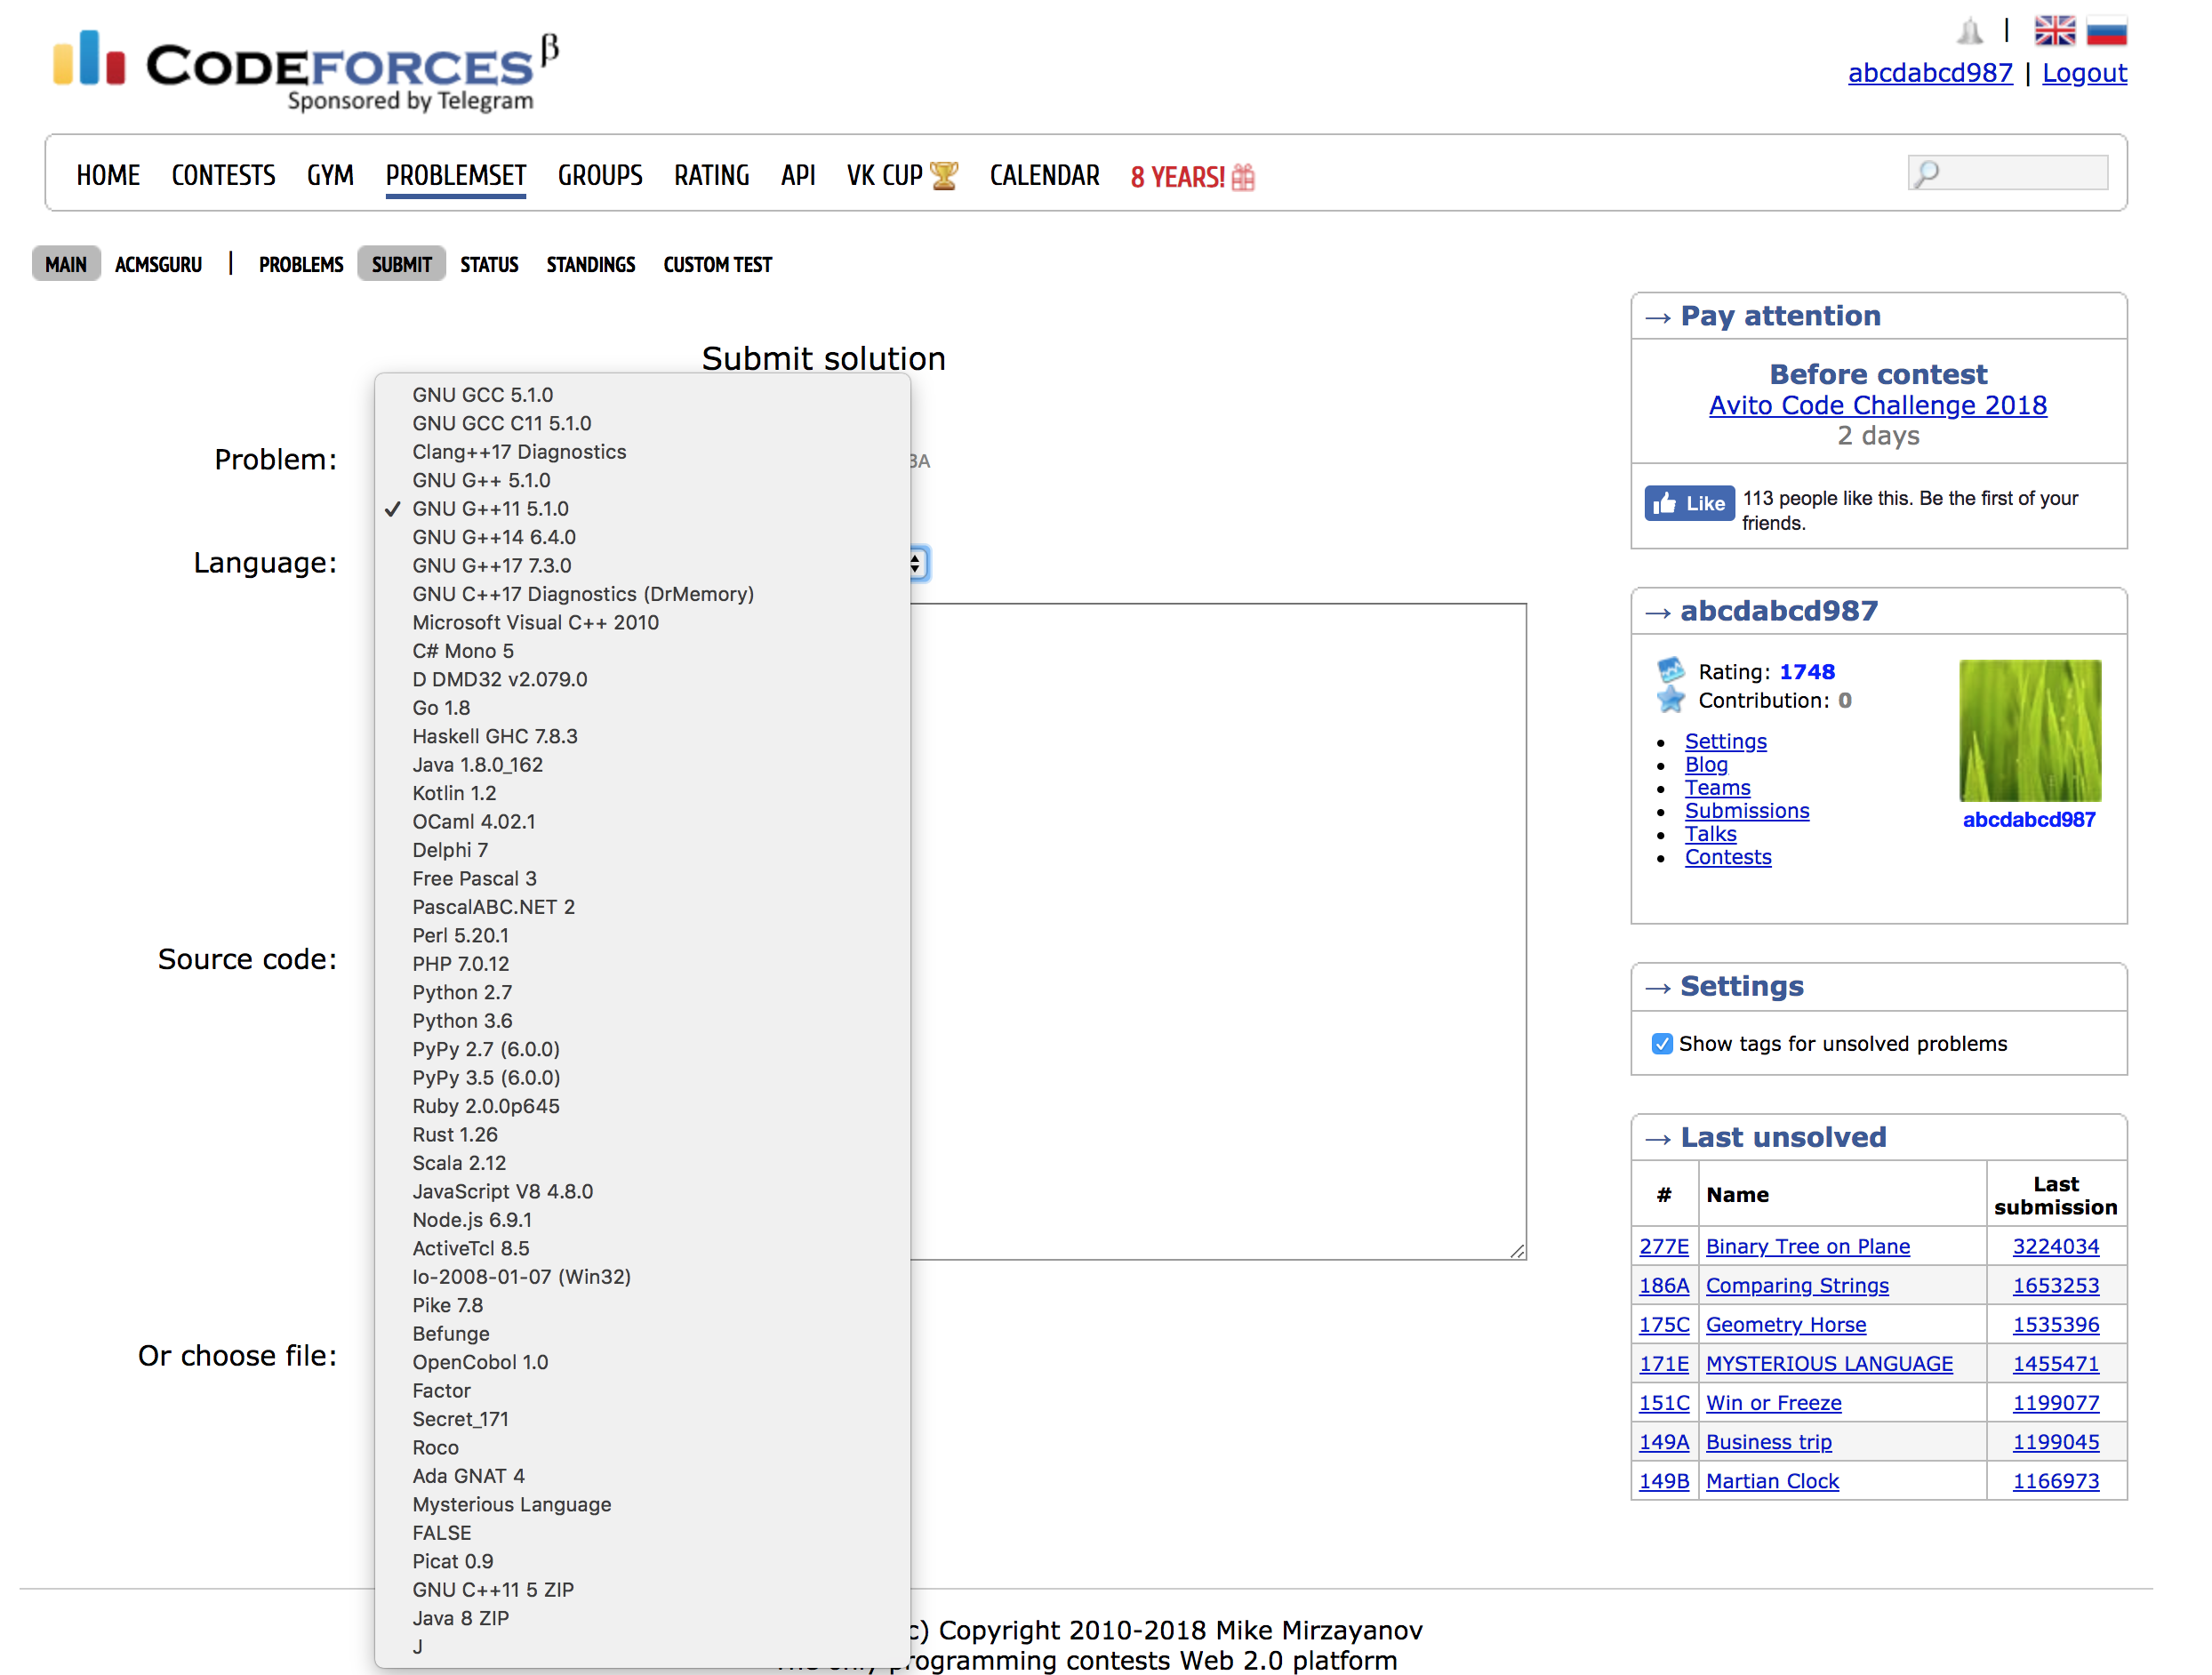
\includegraphics[width=0.8\textwidth]{img/codeforces-languages.png}
                \caption{CodeForces supports a large number of programming languages}
                \label{fig:codeforces-languages}
            \end{figure}

            Recently, \texttt{cgroups} and Linux namespaces features enables operating system level virtualization.
            Container technologies like \emph{LXC} and \emph{Docker} make limiting resources easier.
            Instead of writing detailed security policy,
            the system administrator of an online judge simply needs to specify the coarse resource limits.
            The execution of malicious code is tolerable inside the container
            because the malicious code can at best corrupt the operating system inside the container
            which is isolated from other containers and the host operating system.
            Containers are lightweight as the spawn time is milliseconds and
            there is no overhead of real hardware virtualization.

            Keep in mind that containers are merely isolation provided by Linux kernel.
            Containers and the host share the same kernel.
            Exploiting kernel vulnerabilities might result in the malicious program escaping from the container.
            \cite{shapira_escape_2017}
            For an extra level of security,
            system administrators might run the automatic grader container inside some virtual machine hypervisor.

            \begin{figure}[htp]
                \centering
                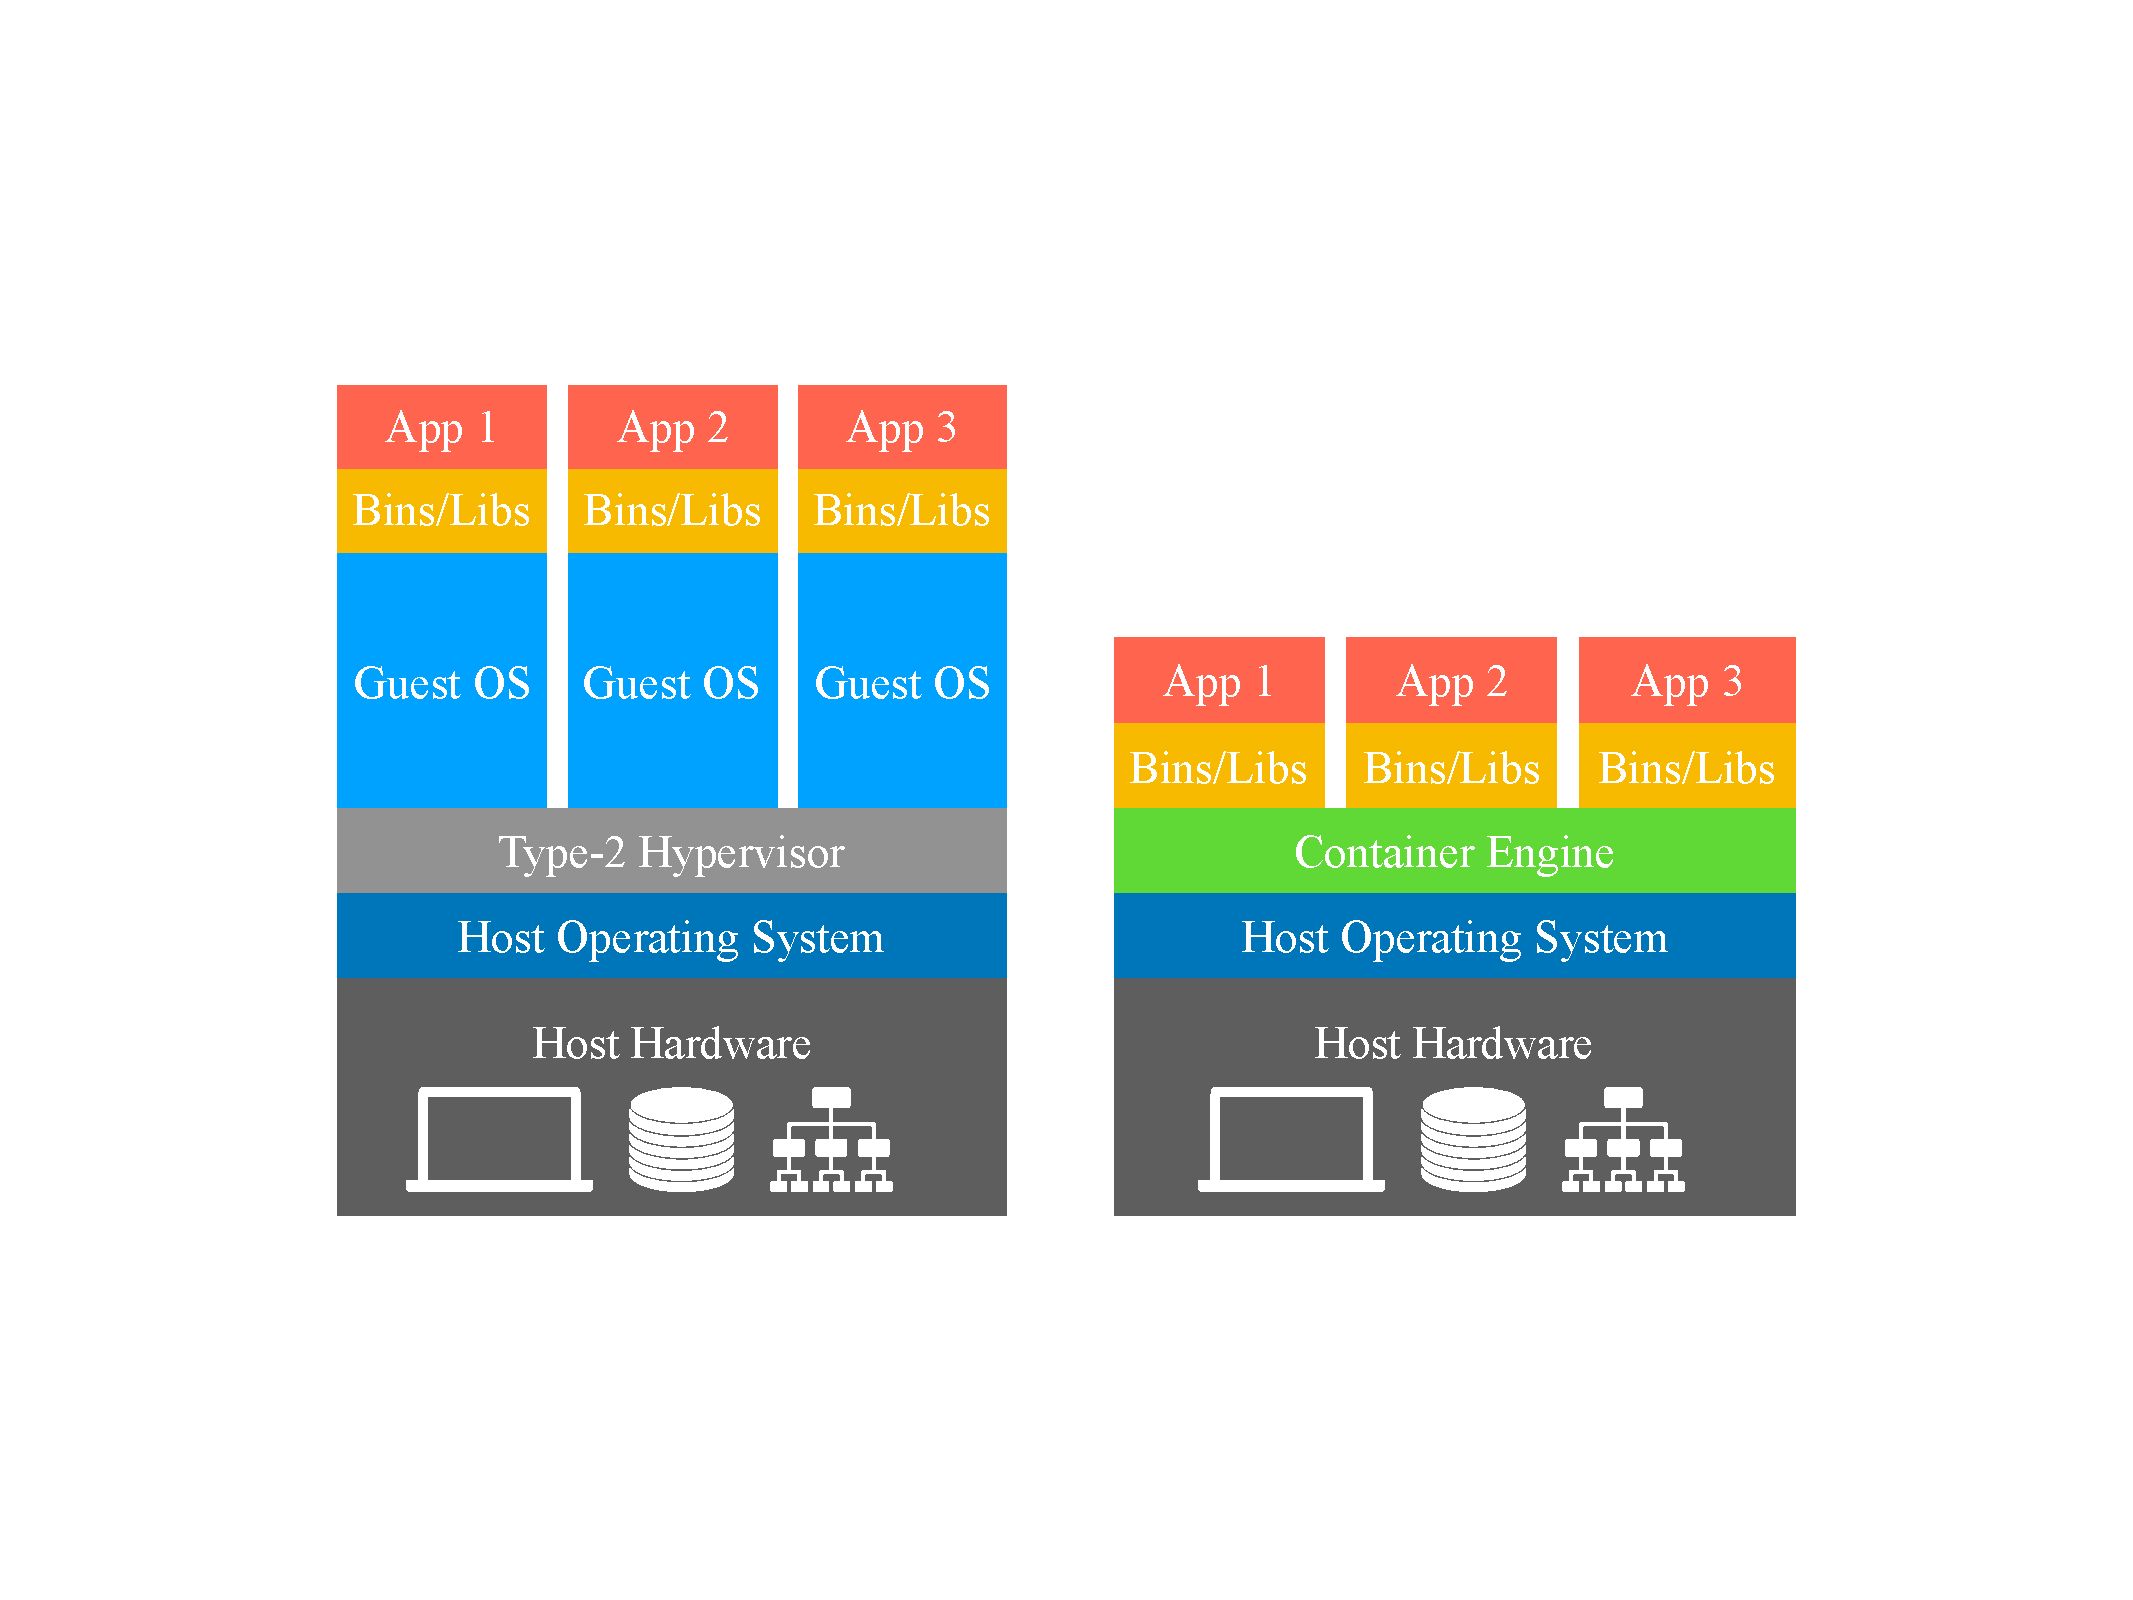
\includegraphics[width=0.8\textwidth]{img/isolation.pdf}
                \caption{Virtual Machine (left) and Container (right)}
                \label{fig:isolation}
            \end{figure}

        \subsubsection{Contests}

            Contest is an important feature of online judges.
            Some online judges, like CodeForces, regularly organize contests,
            attracting thousands of participants of competitive programming competitions.

            A contest consists of a set of problems
            which are usually kept secret before the contest starts.
            A typical contest lasts a few hours.
            Participants can solve the problem set on their own in arbitrary order.
            There is a scoreboard displaying the real-time score of all participants.
            The scoring rule varies.
            Most of the scoring rules sort the scoreboard by the number of accepted solution.
            In order to rank among participants who have solved the same number of problems,
            some rules take the sum of submission time into account, as the second sort key.
            The ACM-ICPC rule also adds extra time penalty to each failure submission.
            The OI rule values partial credits.
            The total score is the sum of credits of all problems, ignoring submission time.

            The ranking system is great stimulation for participants.
            Figure \ref{fig:codeforces-rating} shows rating changes on CodeForces of a user called \texttt{tourist}.
            Online judges with ranking systems update each participants ranking score
            after the contest has finished.
            The ranking systems are usually variants \cite{bailey_algorithm_2018,mirzayanov_open_2015}
            of the Elo rating system \cite{elo1978rating}.
            It takes two factors into account:
            the participant's current ranking and the ranking of other participants.
            It roughly reflects a participant's level.

            \begin{figure}[htp]
                \centering
                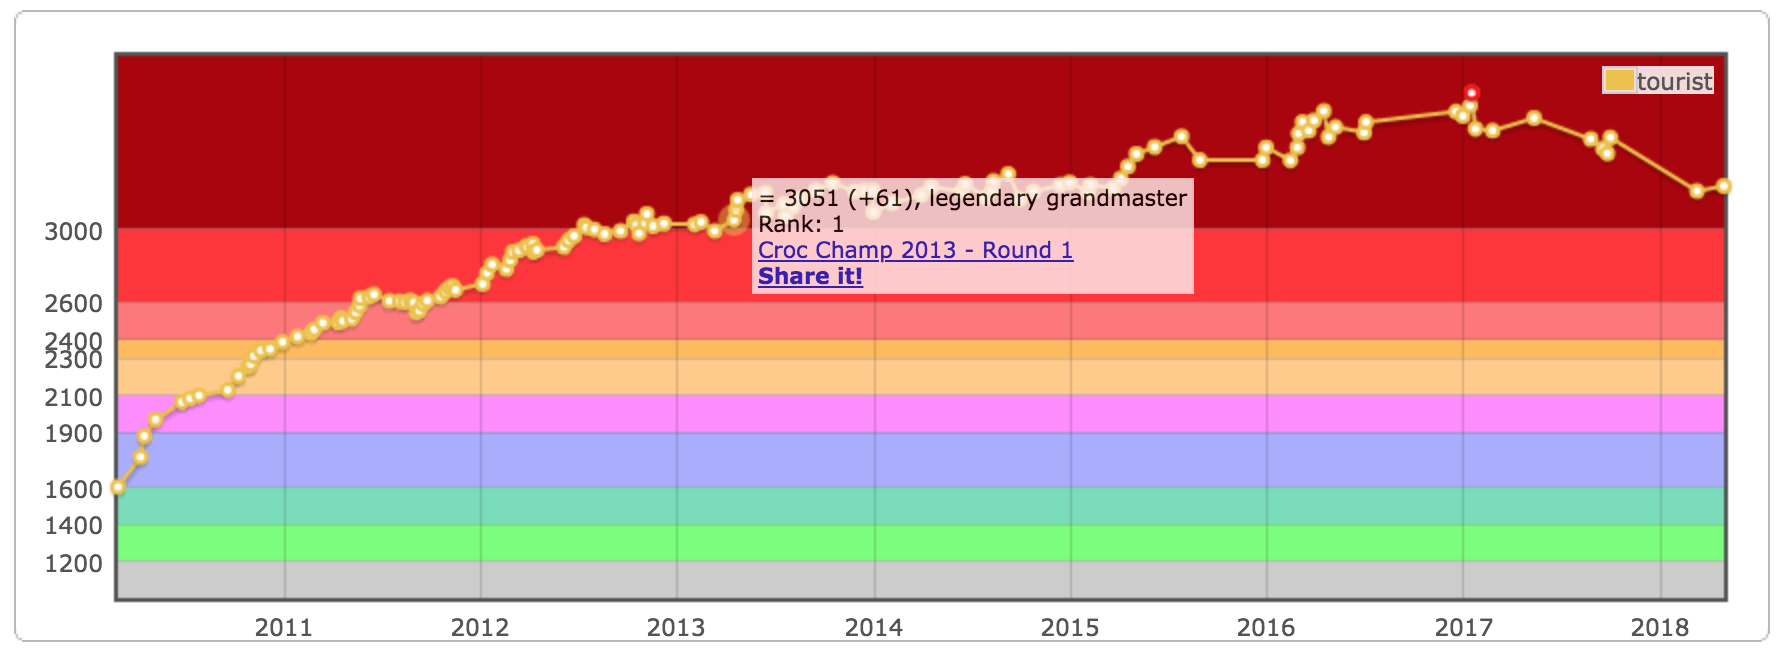
\includegraphics[width=0.8\textwidth]{img/codeforces-rating.png}
                \caption{Rating changes on CodeForces of a user called \texttt{tourist}.}
                \label{fig:codeforces-rating}
            \end{figure}

            The contest feature can also serve other purposes.
            For example, teachers can hold an exam on the online judge
            and ask students to take the exam on a computer room in a planned time.
            Another useful variant of the contest feature is homework.
            Teaching assistants can hand out the problem set on the online judge,
            set the start and end date (which usually spans days or a few weeks).
            The scoreboard precisely shows whether a student has finished all the assignments.

        \subsubsection{Virtual Judge}

            High-quality problems span different online judges.
            Sometimes, students might need to register a new account on a newly visited online judge
            just in order to solve a few assignments.
            Sometimes, tutors of competitive programming competitions might want to organize an exam
            of which problems are from different online judges,
            some of which does not even have a contest feature.
            To deal with these issues, the virtual judge \cite{vjudge} creates a problem-centric platform,
            breaking the boundary of different online judges.

            \begin{figure}[htp]
                \centering
                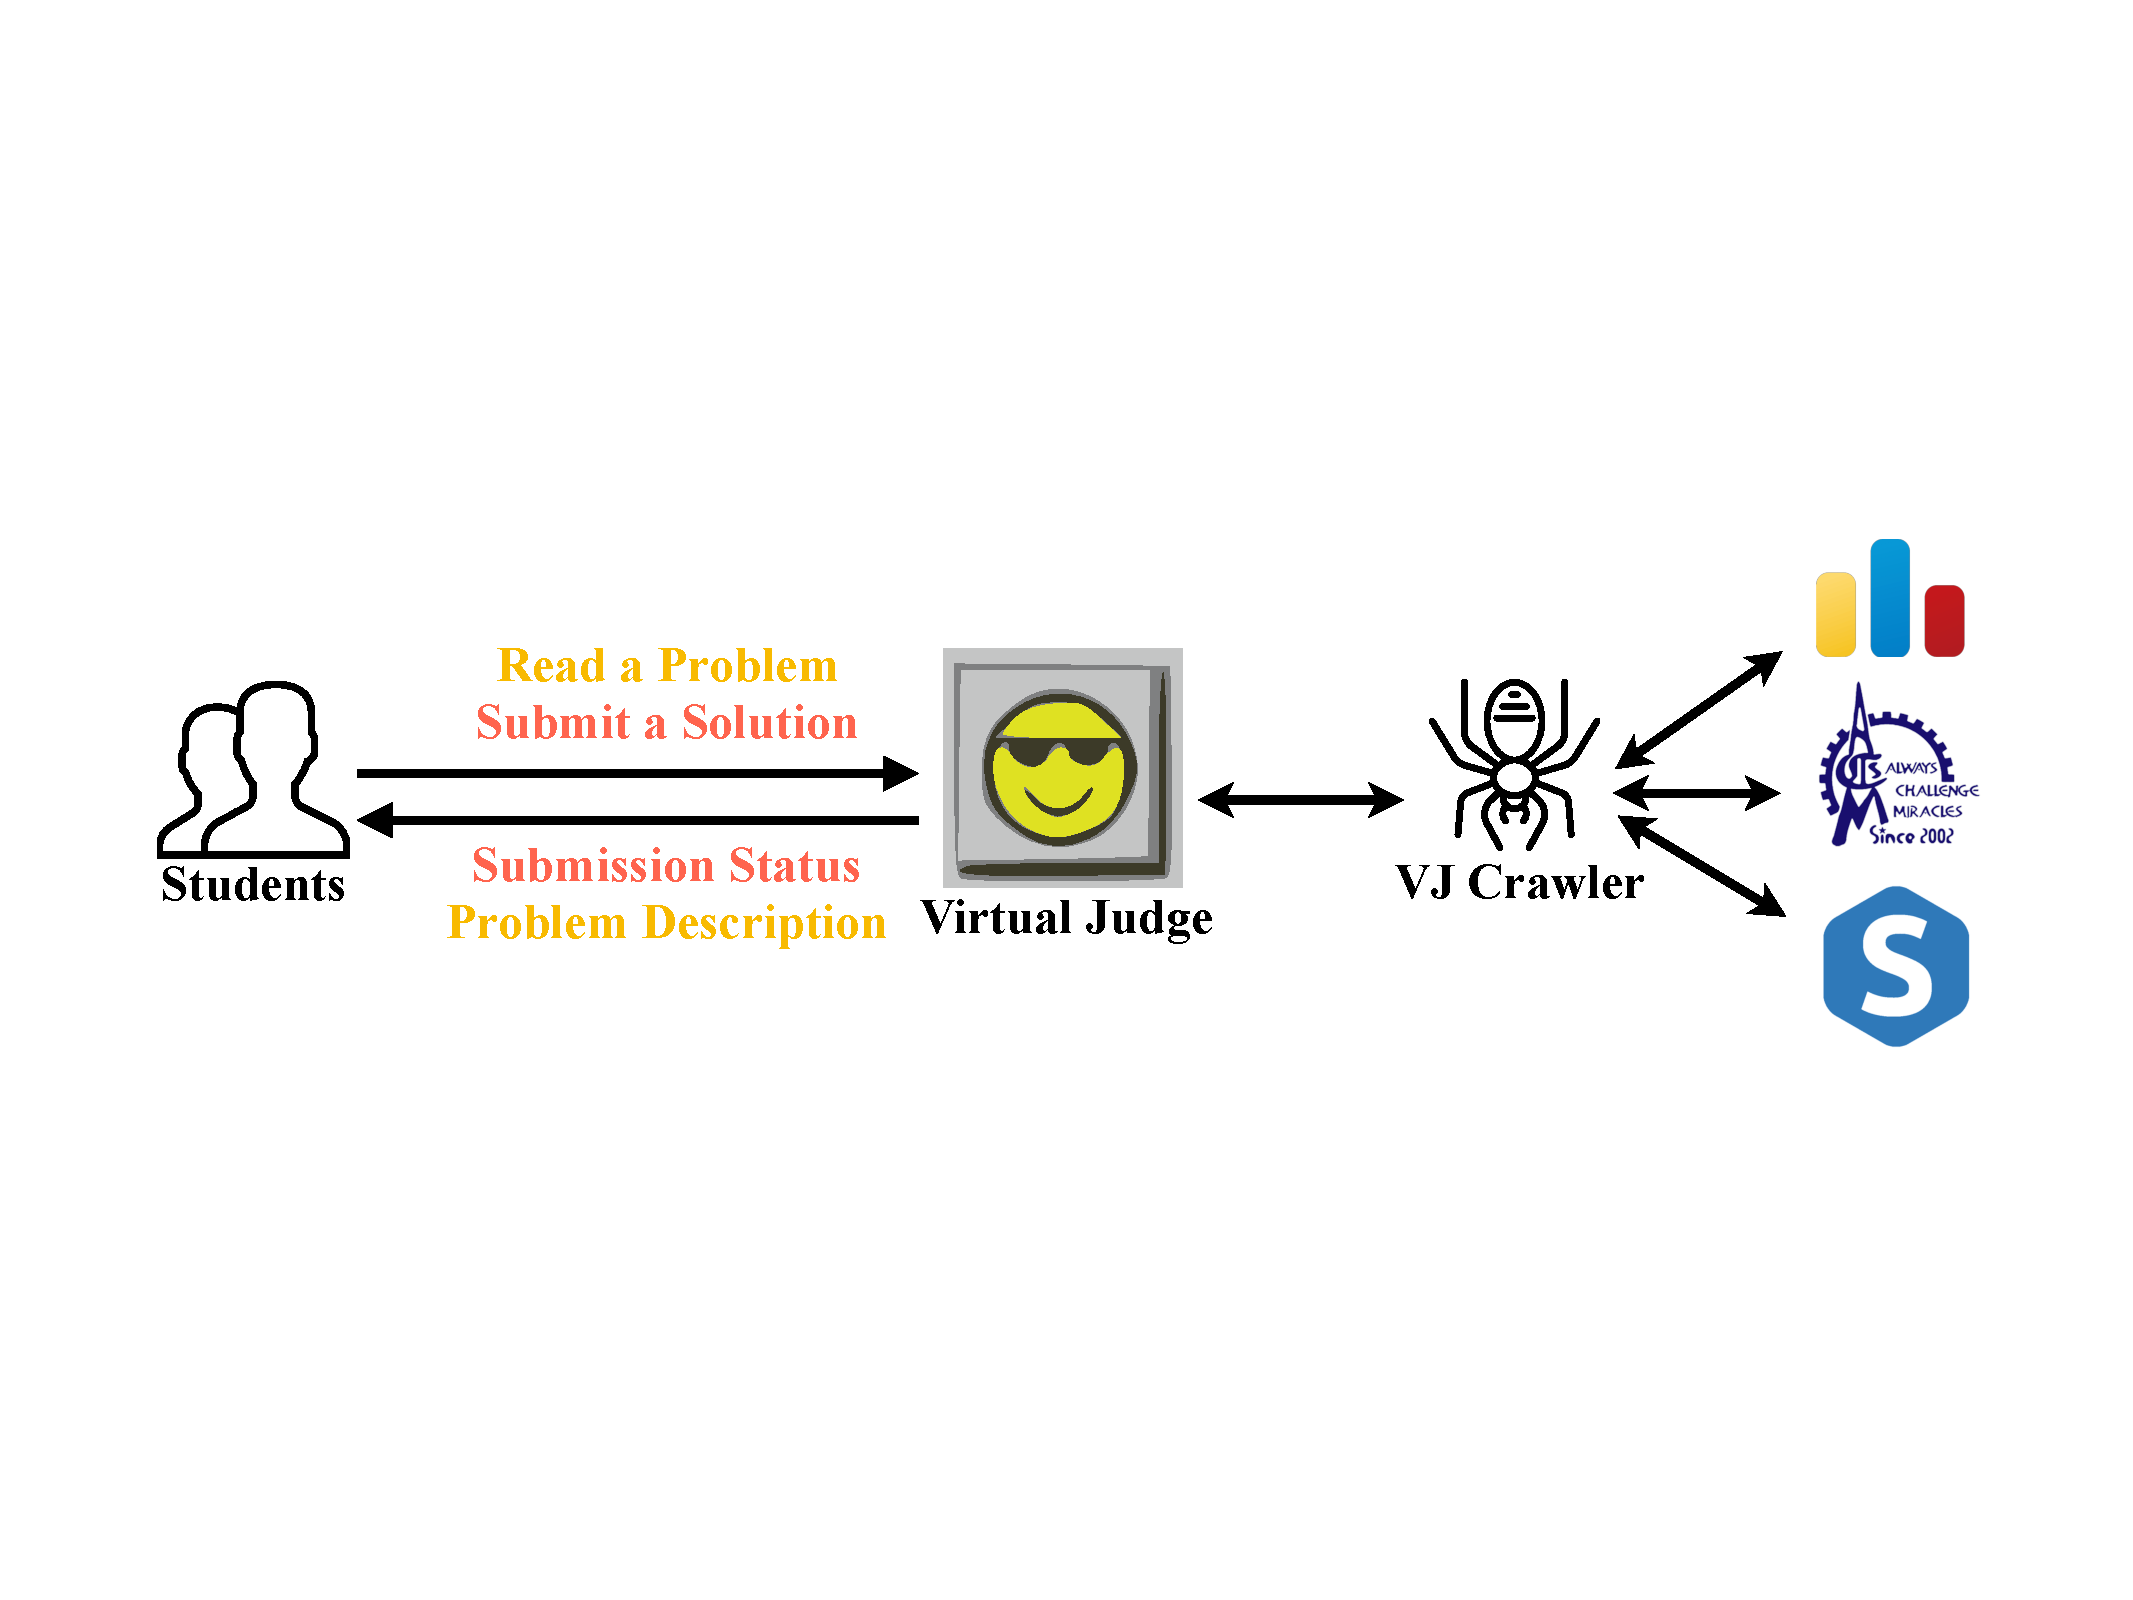
\includegraphics[width=0.8\textwidth]{img/vjudge.pdf}
                \caption{Diagram of virtual judge}
                \label{fig:vjudge}
            \end{figure}

            The ``virtual'' judge is not a ``real'' judge in the sense that it does not own any problems,
            nor does it run any automatic graders.
            It acts like a proxy between students and different online judges (See Figure \ref{fig:vjudge}).
            The virtual judge has a web crawler that retrieves problem descriptions from different online judges.
            Students can then read all problems across different online judges within the same website.

            Students only need to register one account on the virtual judge.
            The virtual judge has several proxy accounts on each online judge.
            When students submit the code to the virtual judge with their own account,
            the virtual judge automatically submit the code to the corresponding online judge
            with the proxy accounts.
            Then, the web crawler keeps watching the status pages of these delegated submissions
            until the result is determined.
            Finally, the virtual judge stores the result fetched by the web crawler to its own database
            and show the result to students.

            The virtual judge also provides a contest feature.
            It does not require the upstream online judge to have a contest feature.
            The virtual judge submits a source code in a contest to the upstream online judge
            as if it is a normal submission.
            The service logic of contest, like submission time period and time penalty, is handled
            by the virtual judge itself.

        \subsubsection{Encouragement in Students' Proactive Participation}

            Once a problem is published on an online judge,
            it is likely that it will always be there in the future,
            because it does not make much sense to take down a problem.
            Therefore, students can see thousands of problems on the online judge.
            If they are willing to try to solve them,
            there is nothing to stop them from doing it.
            They can submit their solutions,
            and the online judge will tell whether it is correct or not.
            It will not require any extra human resources to grade the solution.
            In fact, active participants of competitive programming competitions usually proactively
            train themselves on online judges.
            They even take part in regular contests which online judges organize.

            With thousands of problems available online, comes another issue:
            students submerged by an overwhelming number of problems usually feel lost
            if they do not have an experienced teacher to tell them which problems to solve.

            Some online judges try to address this issue by creating lists of problems
            categorized by the knowledge components that problems need.
            These lists are usually created by teachers,
            whom themselves create the list in an ad-hoc manner
            according to their years of teaching experience.

            Although teachers' experience is precious,
            we must notice that each student is unique.
            They have different mindsets, different ways to understand knowledge,
            and different levels of knowing each knowledge components.
            We expect with the development of artificial intelligence
            and exploitation of millions of submissions data,
            online judges can design unique training problem set for each student.


\section{Machine Teaching}

    Machine learning and deep learning have shown their excellent accuracy and generalization capability
    in many areas including computer visions, natural language processing, speech recognition, and so on.
    However, to train a machine learning model requires experts in machine learning.
    The demand of machine learning model exceeds the supply of ``teachers'' that are able to teach machines.
    In contrast to the machine learning field which focuses on performances like accuracy,
    the machine teaching field pays attention to the efficacy of the teachers given the learners,
    enabling more people like data scientists and domain experts to teach machine learning algorithms,
    the number of which can be hundreds of times more than the number of machine learning experts \cite{Simard2017}.

    A ``teacher'' in machine teaching field aim to design the optimal training set $D$
    to teach a given ``learner'' $A$ a specific model $\theta^*$.
    The definition of ``optimal'' varies.
    For instance, it can be the size of the training set.

    \begin{figure}[!htp]
        \centering
        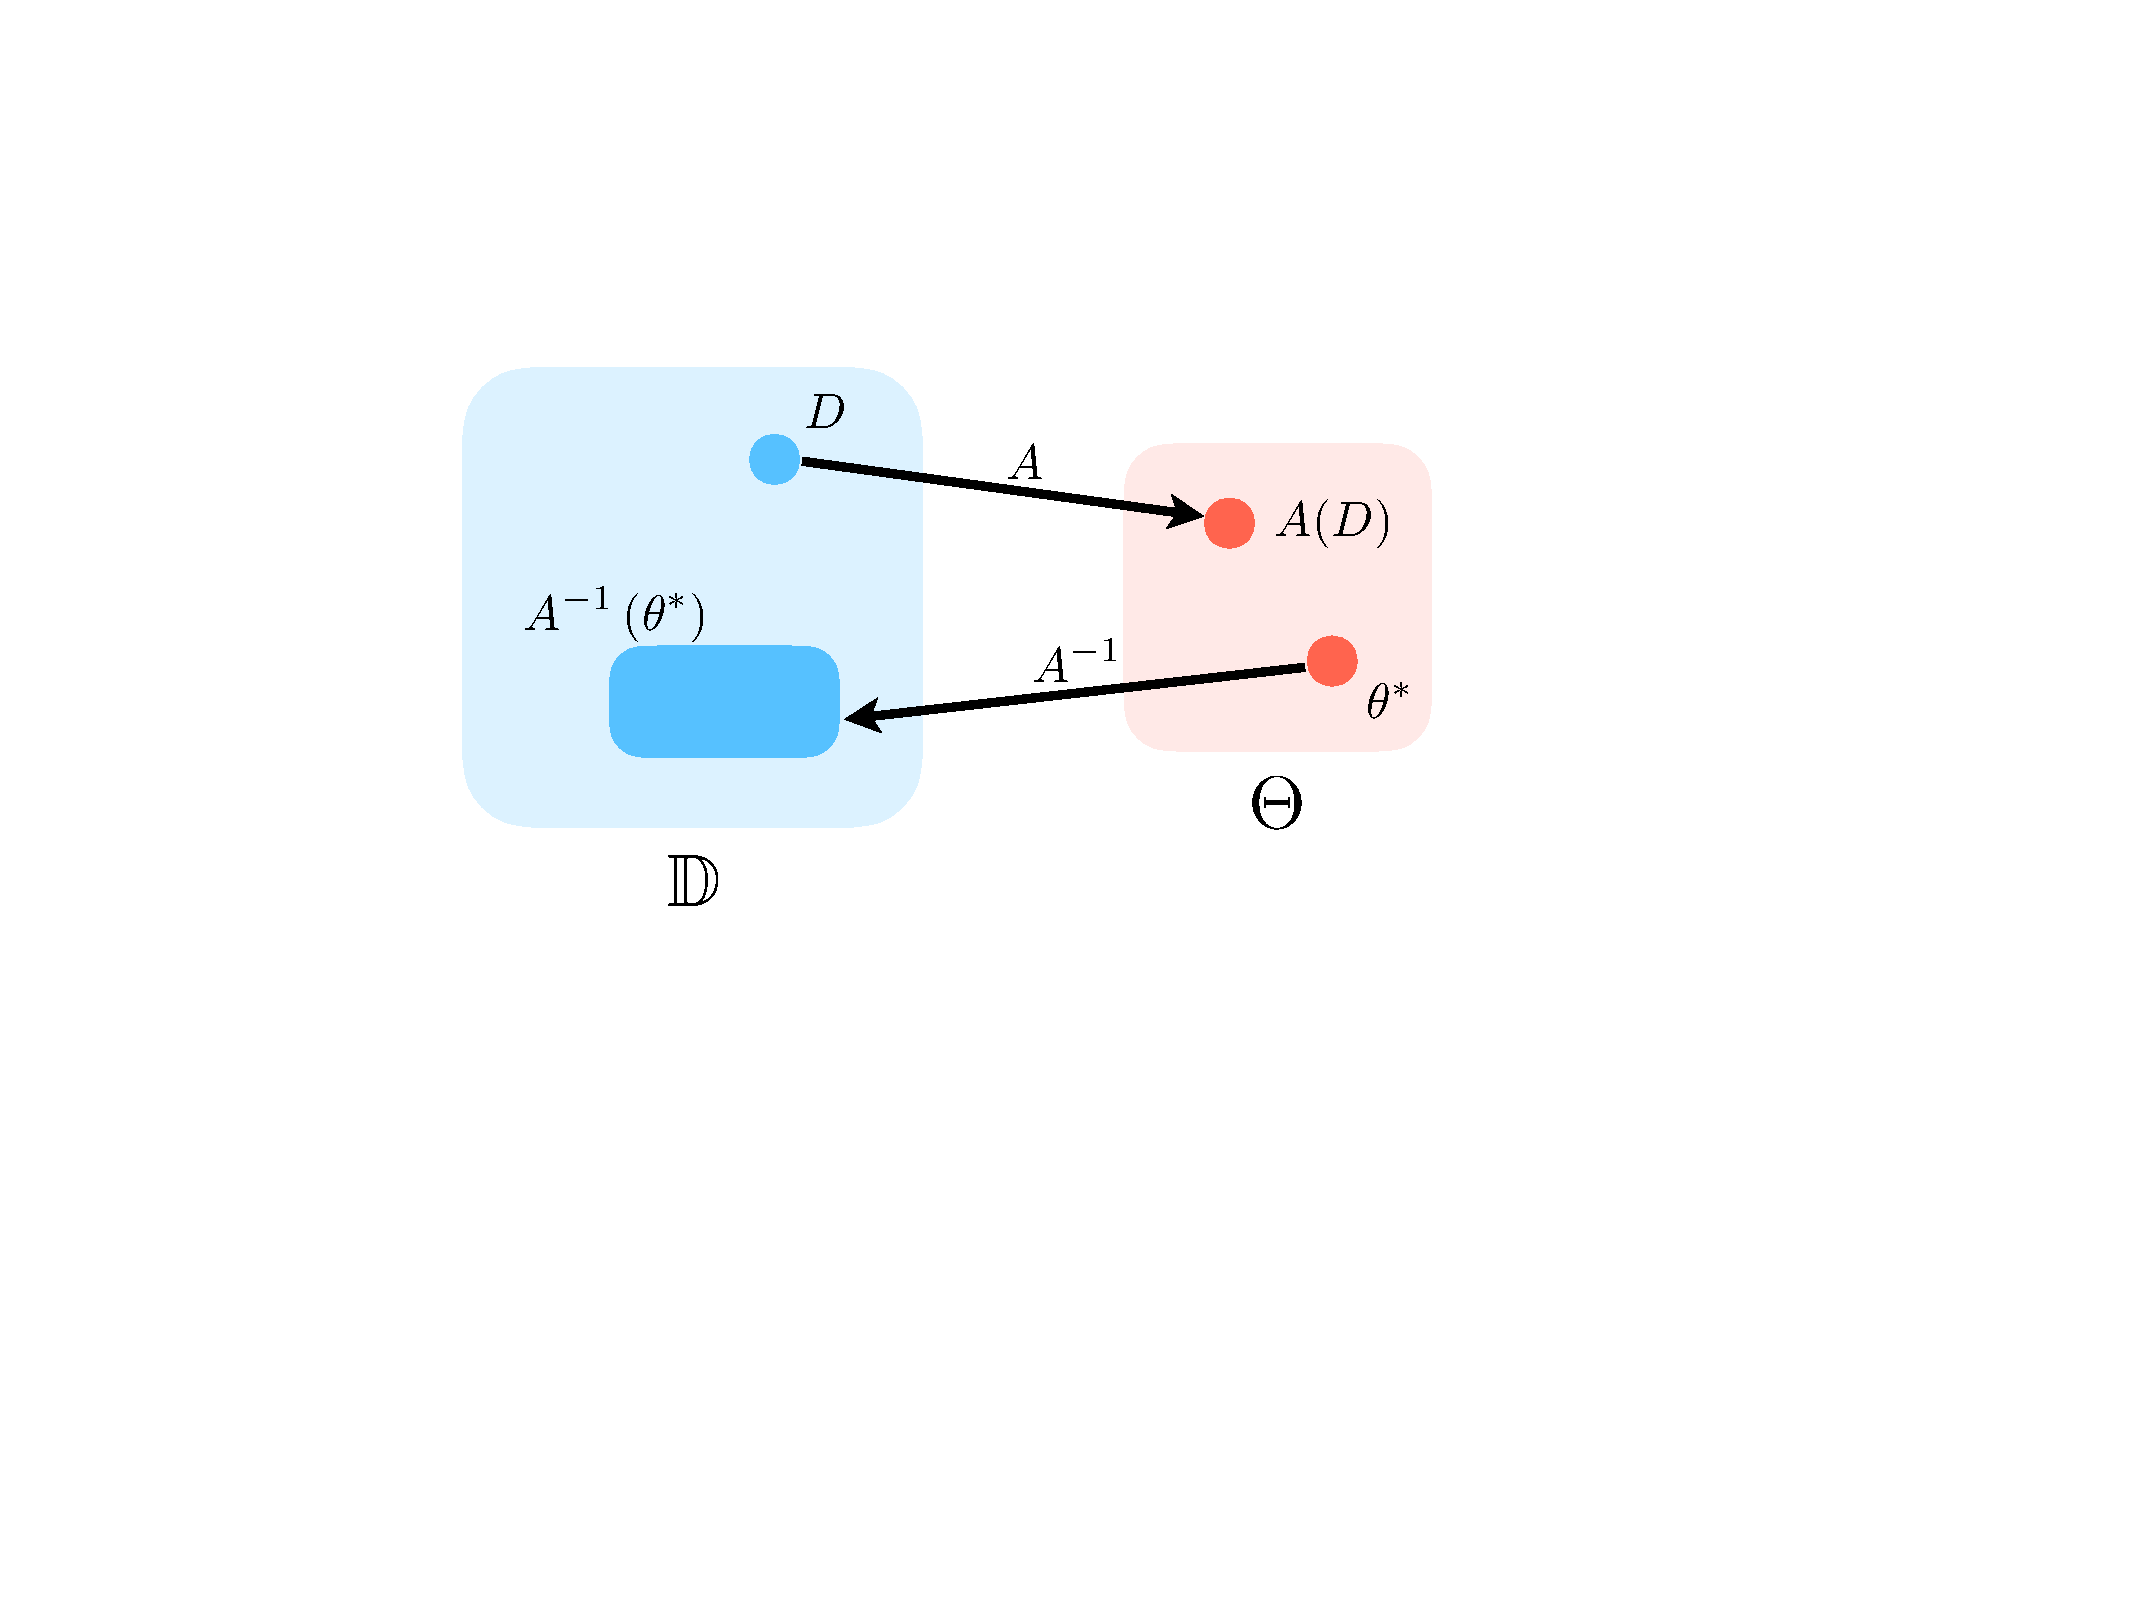
\includegraphics[width=0.4\textwidth]{img/machine-teaching-vs-machine-learning.pdf}
        \caption{Machine Teaching vs. Machine Learning.}
        \label{fig:machine-teaching-vs-machine-learning}
    \end{figure}

    \cite{Zhu2018} views machine teaching as an inverse problem to machine learning.
    Given $D \in \mathbb{D}$ and $A \in \mathbb{A}$, machine learning results in a model $A(D) \in \Theta$.
    Given $\theta^* \in \Theta$ and $A \in \mathbb{A}$,
    there is a subspace $A^{-1}(\theta^*) \subseteq \mathbb{D}$ of training set space. 
    Training $A$ with training set inside $A^{-1}(\theta^*)$ results in the target model $\theta^*$.

    Although a ``teacher'' knows $\theta^*$,
    it is likely that the ``teacher'' cannot directly ``hard wire''the ``learner''
    because they are usually not the same type of entities.

    Machine teaching applications can look entirely different depending who teaches whom.

    \subsection{Human teacher teaches machine learner}

        Machine learning experts who have a deep understanding of the learner algorithm
        and human experts in the learner's domain can design the optimal training set
        boosting the training efficiency of the learner.

        Consider a one-dimension threshold classifier.
        The input distribution is uniform over the interval $[0,1]$.
        Denote the true threshold as $\theta^*$.
        The label is binary and noiseless: $y := \bm{1}_{x \geq \theta^*}$.

        Passive learning receives $n$ training items
        $x_1, x_2, \cdots, x_n \sim U[0,1]$ with $y_i = \bm{1}_{x \geq \theta^*}$.
        It can be shown that with large probability a consistent learner (one that makes zero training error)
        incurs a generalization error $\left|\hat{\theta} - \theta^*\right| = O(n^{-1})$ \cite{Zhu2018}.
        The uncertainty of the decision boundary is defined by the innermost pair of negative and positive samples.
        Equivalently, archiving $\epsilon$ error requires $n \geq O(\epsilon^{-1})$ training data.

        A human teacher knows $\theta^*$ can construct a training set containing only two items
        that are $\epsilon$ apart with $\theta^8$ in the middle.
        Training on this two-item training set results in $\epsilon$ generalization error for any $\epsilon$.

        Study shows that in the case that human teacher is not able to give the optimal training set,
        machine teaching allows the machine student to ``teach the human how to teach'' \cite{Suh2016}.

    \subsection{Machine teacher teaches machine learner}

        An adaptive spam filter $A(D)$ are constantly re-train over time on training set $D$ to accommodate
        the changing legitimate content and the variants of spams.
        The machine learner can be a malicious program that sends specially designed emails
        to the spam filter to manipulate the threshold from $\hat{\theta}$ to some nefarious $\theta^*$ instead,
        such that certain spam emails can get pass the filter \cite{Alfeld2016}.
        The machine learner changes the training set of the spam filter subtly by $\delta$ to avoid detection \cite{Mei2015}.
        The attacking problem can be formalized as:

        \begin{equation*}
        \begin{aligned}
            \min_{\delta, \hat{\theta}} \quad &
            \left\lVert\hat{\theta} - \theta^*\right\rVert + \eta \left\lVert\delta\right\rVert \\
            \textrm{s.t.} \quad & \hat{\theta} = A(D+\delta)
        \end{aligned}
        \end{equation*}

    \subsection{Machine teacher teaches human learner: Education}

        Every human student is unique.
        They have different mindsets, different skill sets, and different mastery over knowledge components.
        Machine teaching provides a unique approach to design the optimal lessons for individual students.

        Machine teaching explicitly assumes a cognitive model $A$ of students.
        Given lessons $D$, we can compute the resulting cognitive state $A(D)$,
        and then evaluate the test score via an appropriate teaching risk function $\rho(A(D), \theta^*)$
        whose minimum is at $\theta^*$.
        In other words, machine teaching treats the human learner as a ``transparent box.''

        Although having a correct cognitive model is a strong assumption,
        machine teaching with inaccurate cognitive model still works on humans \cite{Whitehill2017}.
        In the work of \cite{Patil2014},
        researchers assumes a limited capacity retrieval cognitive model of human learners
        in a one-dimension classification task.
        Human testers trained on the training set the machine teaching method designed
        has statistically significantly better test accuracy than who trained on a random training set.














